\chapter{Mbona Hatcheries Records}


\section{Record Keeping}

The various record keeping forms appear in the appendix of this document. The forms are self explanatory.
Eventually the Appendix will also contain records from years gone by if they still exist. 

\subsection{Season starting June 2018}

The 2018 season started with the arrival of $10000$ eyed Rainbow Trout eggs from the Underberg Hatchery. 
The temperature of the water at the Underberg hatchery was approximately \SI{12}{\celsius}.
The eggs arrived at Mbona at14h30 in two trays with one ice tray on the bottom and 
another ice tray on the top of the transportation cooler box.

On arrival at Mbona the temperature of the eggs in the top tray was \SI{12}{\celsius} which was brought up to
the Mbona water temp of \SI{14.6}{\celsius} by 16h00 and these eggs were then moved to bath B.

On arrival at Mbona the temp of the bottom tray was \SI{10}{\celsius} 
which was brought up to Mbona water temp of \SI{14.6}{\celsius} by 16h30 and these eggs were placed
in bath A.

Once the eggs had been transferred to the incubation baths, the process of removing dead eggs began.
In table ~\ref{tab:Incubation2018} we show how many dead eggs were removed from each bath per day
during the incubation period.

Feeding the Rainbow fry with fish food starter powder commenced on Tuesday the $12^{th}$ of June.

On Thursday the $14{th}$ of June a further $3000$ brown trout eyed eggs from the Trova Trout company 
in Sabie arrived at the Mbona Hatchery. These ova were packed in iced trays and air freighted to PmB. 
They arrived at Mbona at 9am at a temperature of \SI{5.1}{\celsius}. 
The temperature of the eggs was gradually increased to \SI{13.1}{\celsius} over a period of 5 hours. 
The ova were transferred to a hatching tray in bath C at 14h00 when the water was at 
temperature \SI{13.4}{\celsius}. 
Removal of dead ova from Bath C commenced on Friday the $15^{th}$ of June, 
see table ~\ref{tab:Incubation2018} for daily mortality counts.

\begin{table}[H]
  \centering
  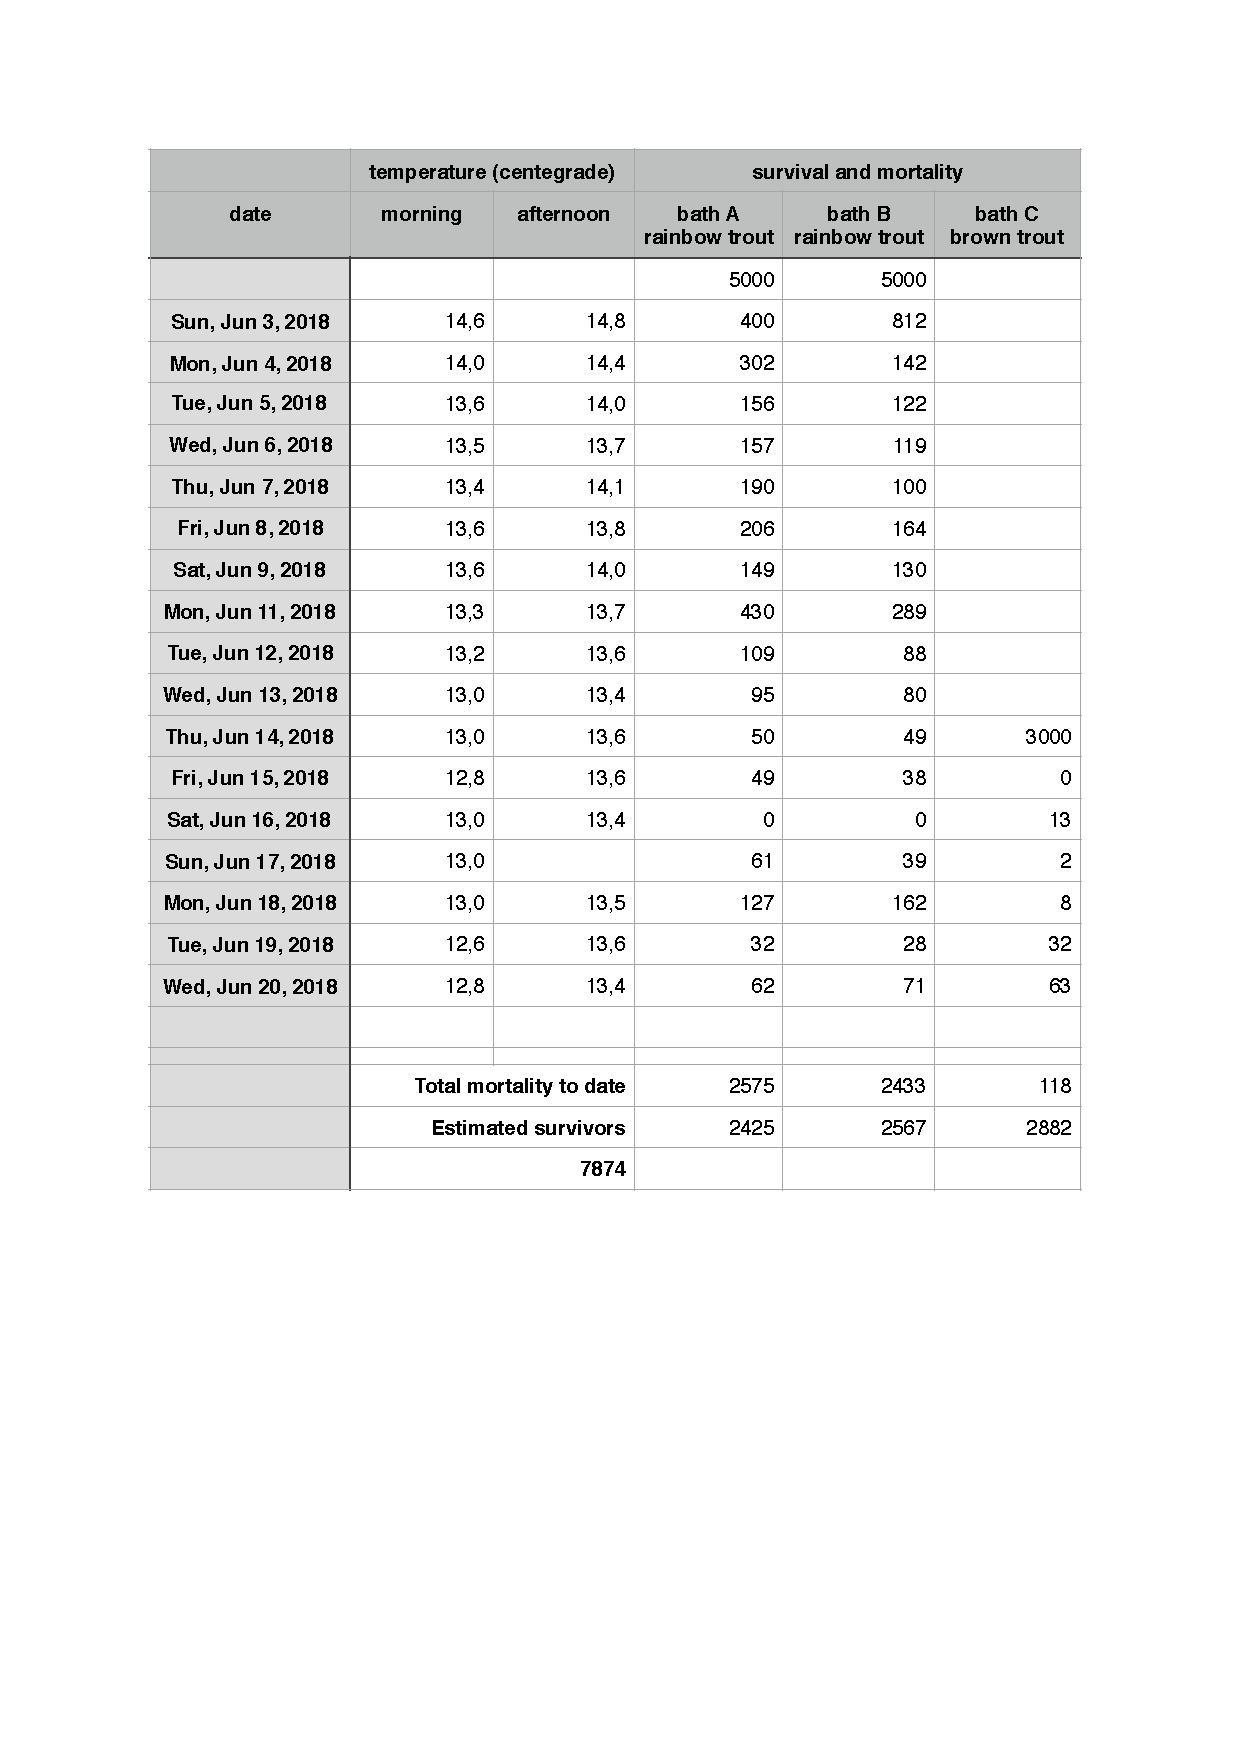
\includegraphics[scale = 0.9]{tables/TablesIncubationMortality.pdf}
   \caption{Temperature and mortality records for 2018 incubation period.}
  \label{tab:Incubation2018}
\end{table}

Assuming that the number of eggs at purchase was accurate and that dead eggs were counted accurately
table ~\ref{tab:FryRelocation2018} suggests that we could expect approximately 5000 surviving Rainbow fry 
ready for relocation to the fry tanks. So we were pleasantly surprised when the Relocation counts as 
shown in table ~\ref{tab:FryRelocation2018} indicated approximately 8000 surviving Rainbow fry.

\begin{table}[H]
  \centering
  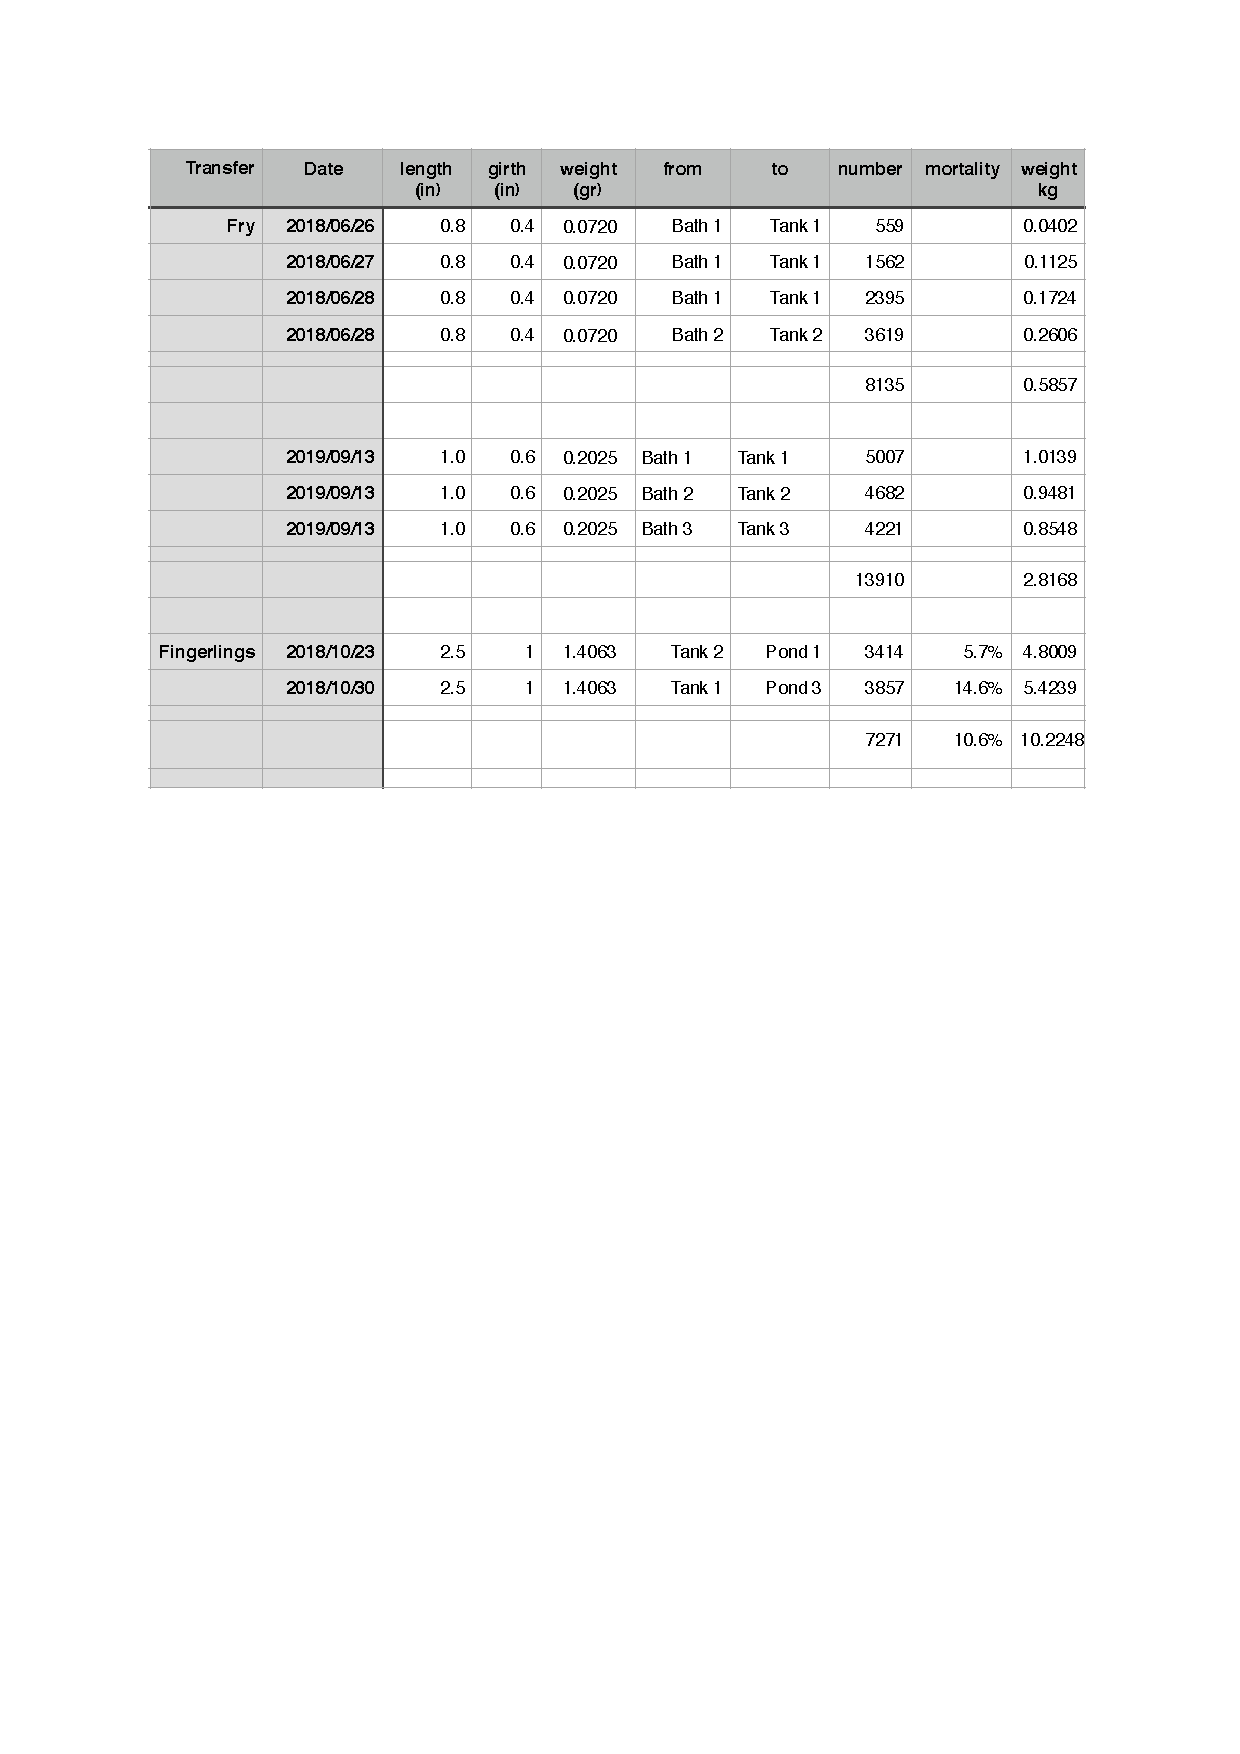
\includegraphics[scale = 0.9]{tables/TablesFryRelocationRecord.pdf}
   \caption{Counts for 2018 relocation of fry from baths to tanks.}
  \label{tab:FryRelocation2018}
\end{table}

This 40\% discrepancy is either due to receiving more eggs than expected or due to the
counting of hatched egg shells as dead eggs or to both.

\subsubsection{Rearing the fry in the tanks}
Two weeks after relocation of fry from baths to tanks we carried out length and weight measurements
on the fry. The results can be seen in table ~\ref{tab:FryGrowth} where the recommended feeding
schedule is given as computed from the suggestions given in chapter 3.

\begin{table}[H]
  \centering
  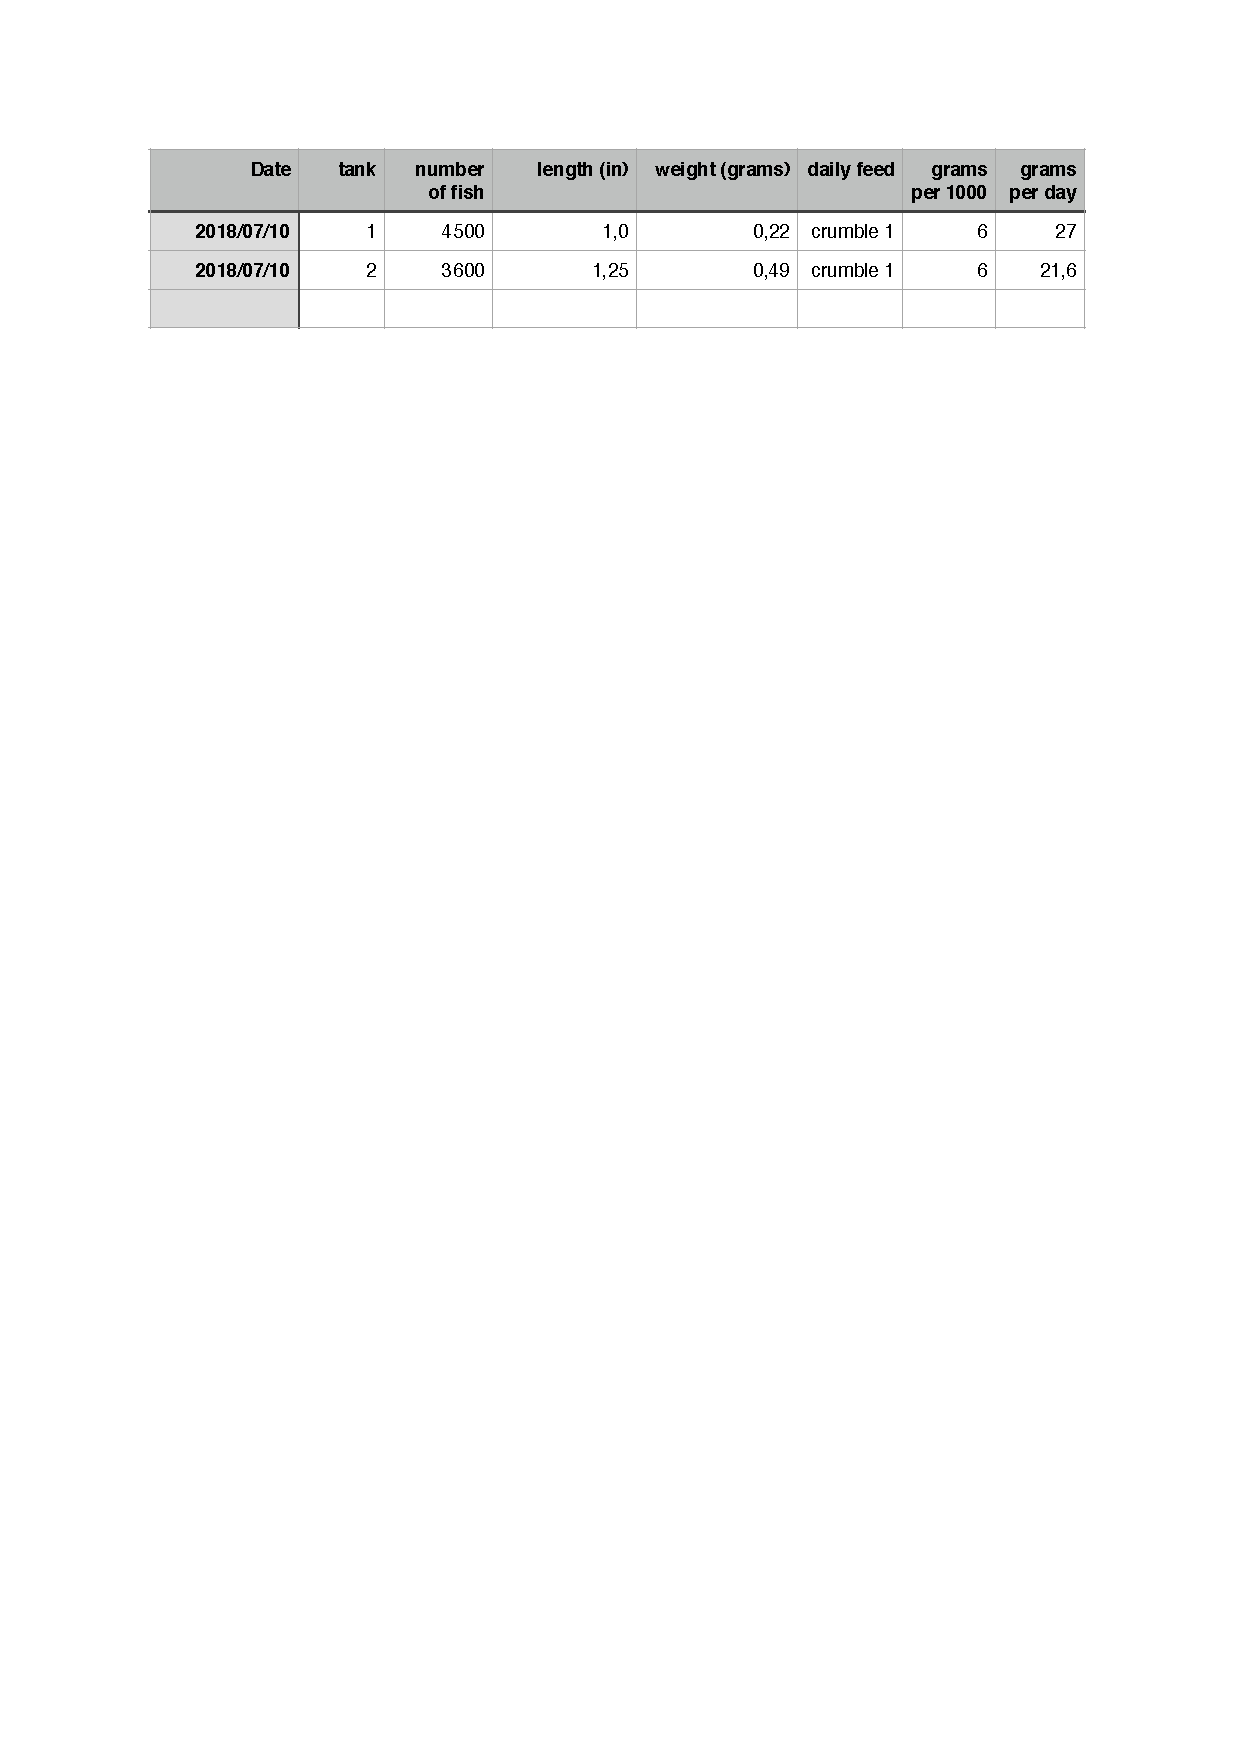
\includegraphics[scale = 0.9]{tables/TablesFryGrowth.pdf}
   \caption{Weight and Length measurements of growing fry}
   \label{tab:FryGrowth}
\end{table}

\subsection{Disposal of Mature Fish}

During the 2018-19 season we sell 2017 fish live to local customers and 
when available, dressed fish to Mbona shareholders. We use the remainder
to stock our dams at Mbona. see tables, \ref{tab:ExternalSales2018}, 
\ref{tab:ShareholderSales2018} and \ref{tab:MbonaDamSales2018} below.

\begin{table}[H]
  \centering
  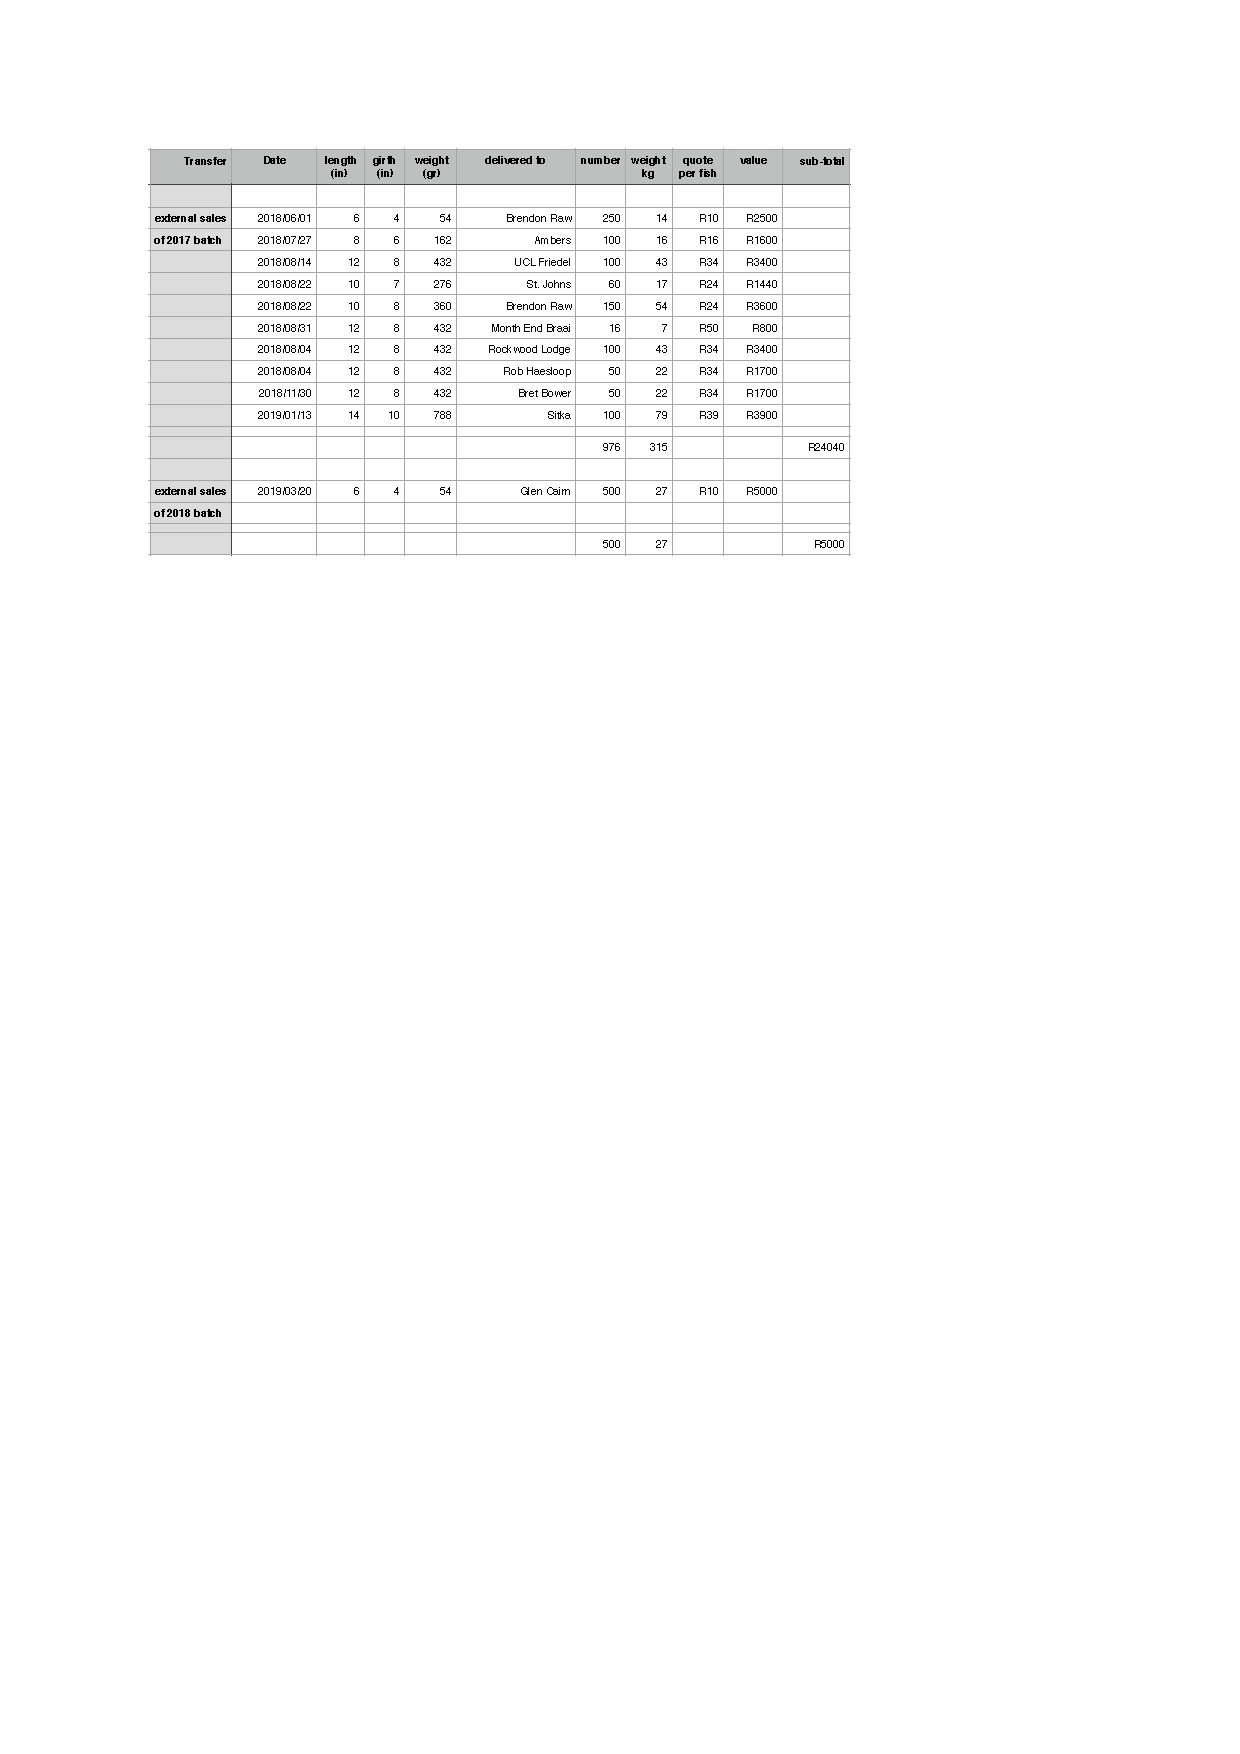
\includegraphics[scale = 1.2]{tables/TablesExternalSales.pdf}
   \caption{2018-19 sales of live fish to external customers.}
  \label{tab:ExternalSales2018}
\end{table}

\begin{table}[H]
  \centering
  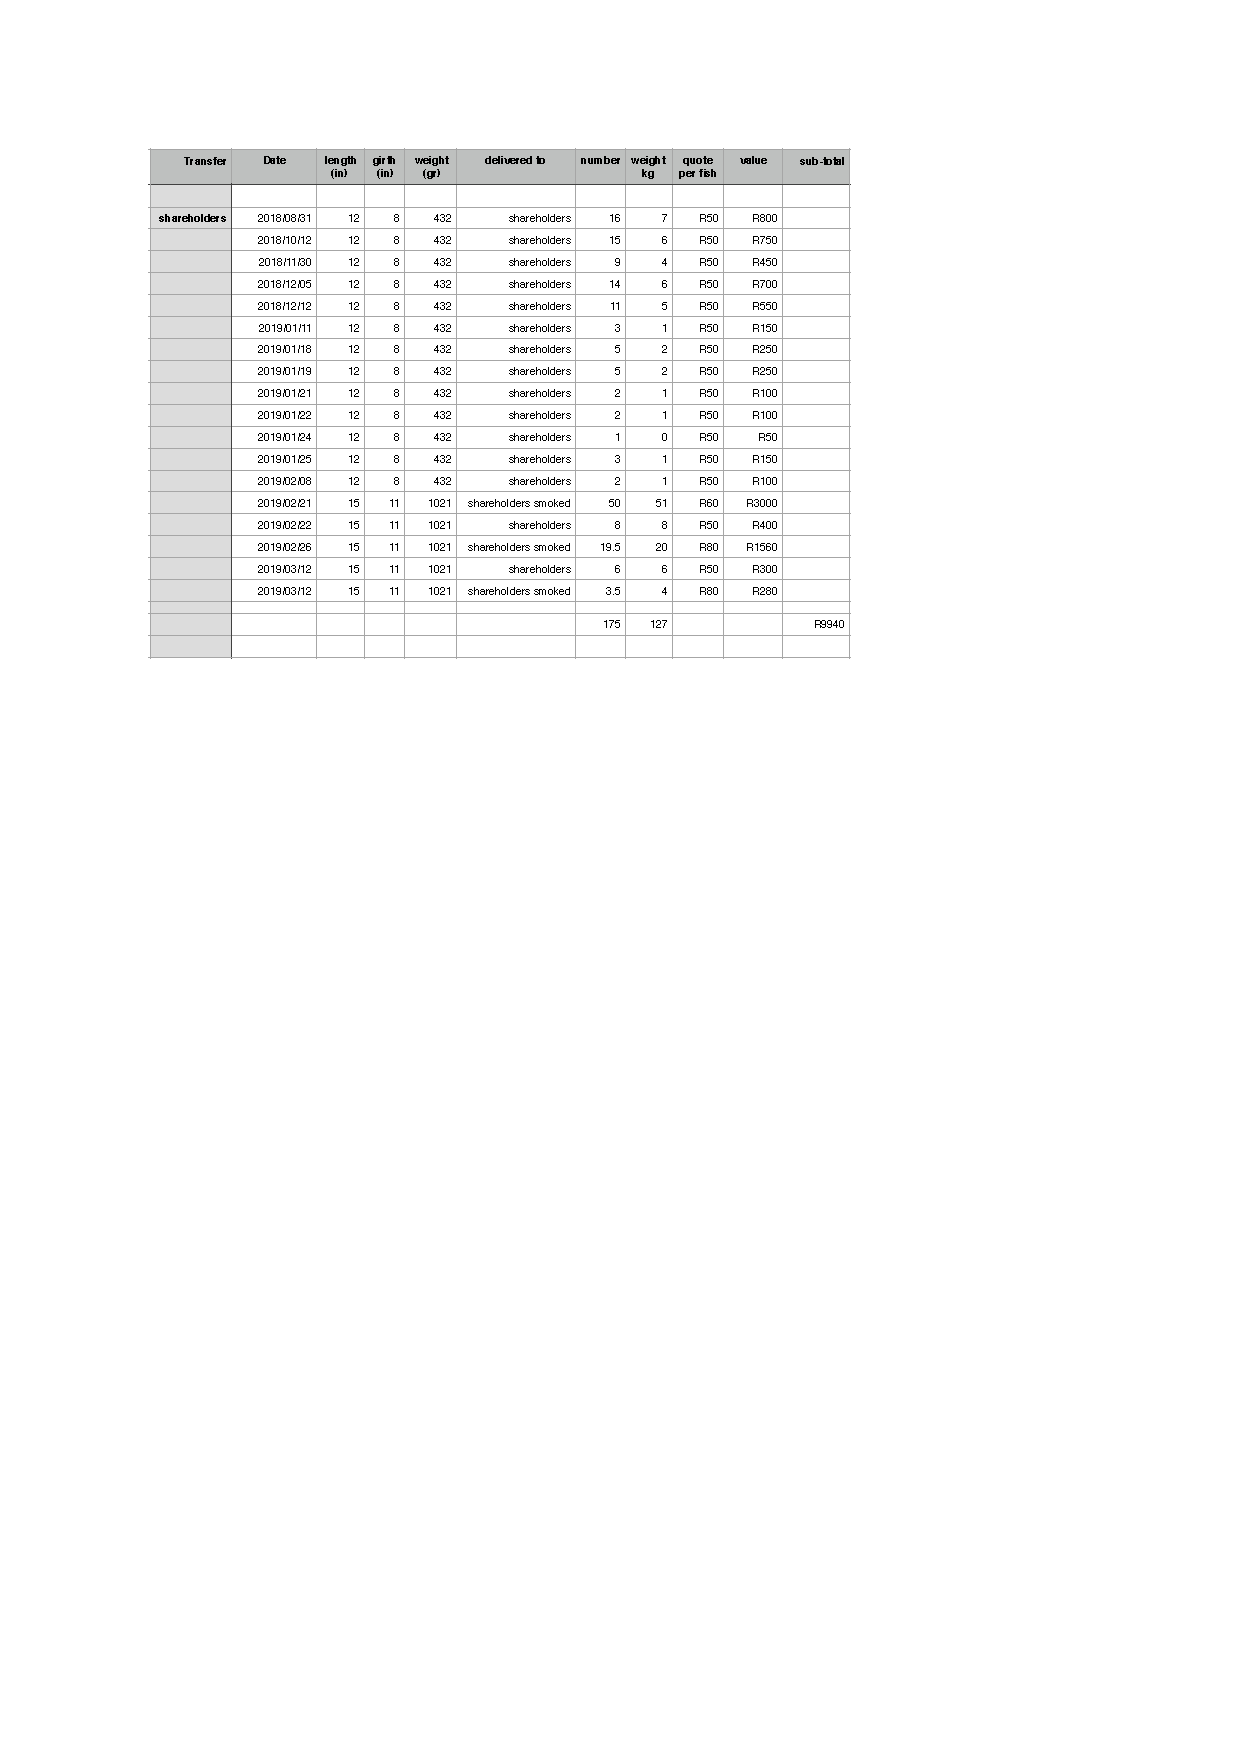
\includegraphics[scale = 1.2]{tables/TablesShareholderSales.pdf}
   \caption{2018-19 sales of dressed trout to Mbona shareholders.}
  \label{tab:ShareholderSales2018}
\end{table}

\begin{table}[H]
  \centering
  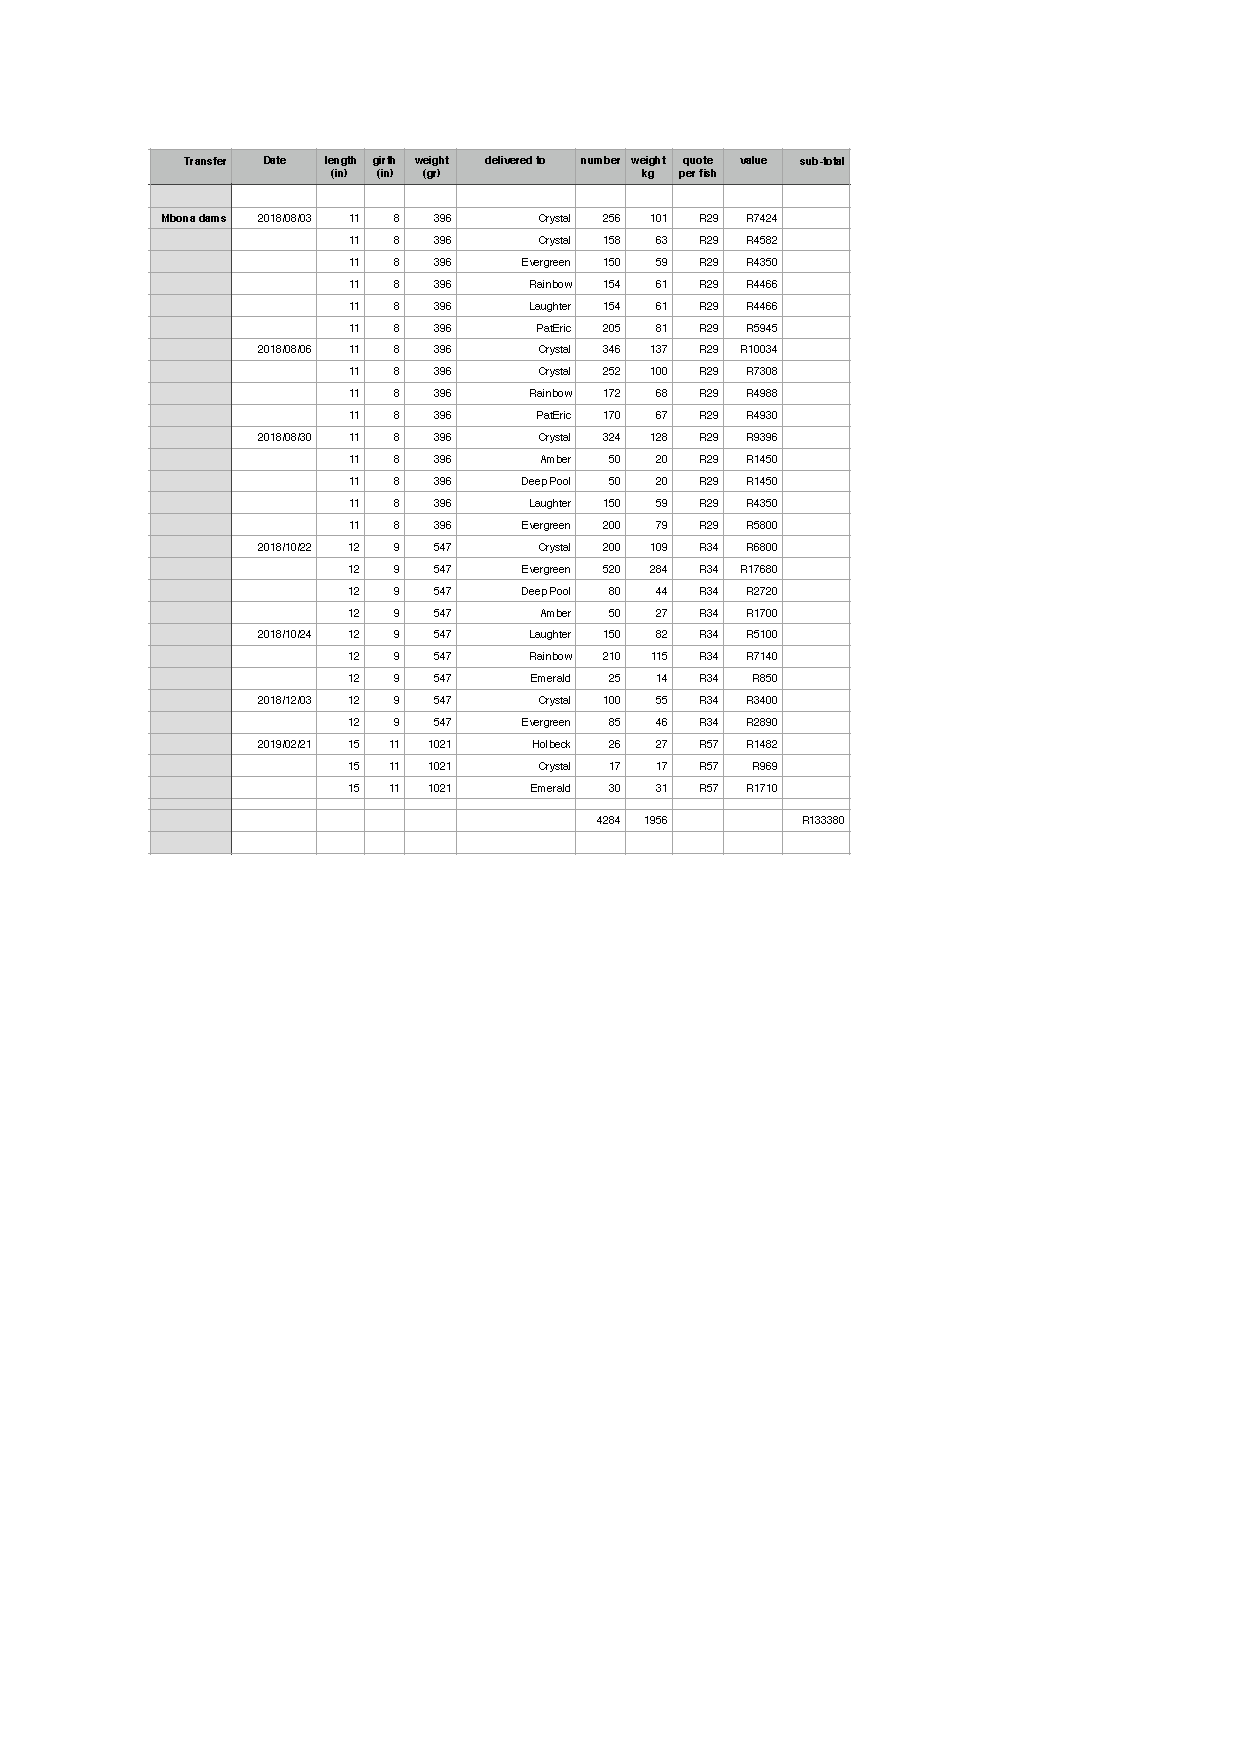
\includegraphics[scale = 1.2]{tables/TablesMbonaDamSales.pdf}
   \caption{2018-2019 stocking of Mbona dams from eggs hatched in 2017.}
  \label{tab:MbonaDamSales2018}
\end{table}


\section{Mbona Hatcheries Maintenance and Repair detail}

Maintainance and repair projects as of July 2018.

\subsection{Hatching room}     

\begin{itemize}
\item Repair bath 2 in-feed pipe
\item Make good all three bath outlets and make adjustable drains. 
\item Make 3 PVC/F-glass mesh filter curtains  
\item Stop leaks in drain out-pipes
\item Sort 220v lighting in hatching room
\end{itemize}

\subsection{new fertilisation cabin}
\begin{itemize}
\item purchase wooden guard hut and install over concrete anti vibration base for egg towers.
\item make solid egg tower table  
\item build new design egg hatching towers.
\end{itemize}


\subsection{Main pond area}     
\begin{itemize}
\item Complete clay repair and gravel of raceway pond.    
\item Complete fencing and gates to new extension   
\item Reroute electric fencing
\item Run water feed pipe to new area off main 3 pond feed
\end{itemize}

\subsection{Shade cloth cover}  
\begin{itemize}
\item Replace and reset gum poles  
\item Re-string or replace 8gg straining wire 
\item Stitch shade cloth to straining wire (wind)
\item Fit 90 degree bend to top of central stand pipe  
\item Replace swimming pool hose sections where necessary
\item Build, using old fencing standards, adjustable drain pipe stands
\item Do 12 volt night light bug catch test with white plastic 
\end{itemize}


\subsection{Syphon water feed from Crystal}
\begin{itemize}
\item  Pull up 2 x 70mm syphon pipes and replace filters
\item Build mud anchor and substantial top float with nylon rope-pulley lifting system for maint.
\item Box and cover 3 x vacuum break valves at Crystal edge for quick access
\item NOTE: Main water pump suction line to be suspended from raft.
\end{itemize}


\subsection{Oxygenator}
\begin{itemize}
\item  Remove IBR roof
\item Remove T from North 70mm pipe and extend  
\item Sort distributor tray or trays
\item Check bottom of bath outlet drain
\item Box and lid 2 x 70mm syphon pipe taps and hose connect points for quick access
\item Extend and secure steel inspection ladder
\item Gravel South side walk area against wall
\item Paint oxygenator
\end{itemize}


\section{Budget proposal}

This section requires further development by the fishing committee.

\begin{table}[H]
  \centering
  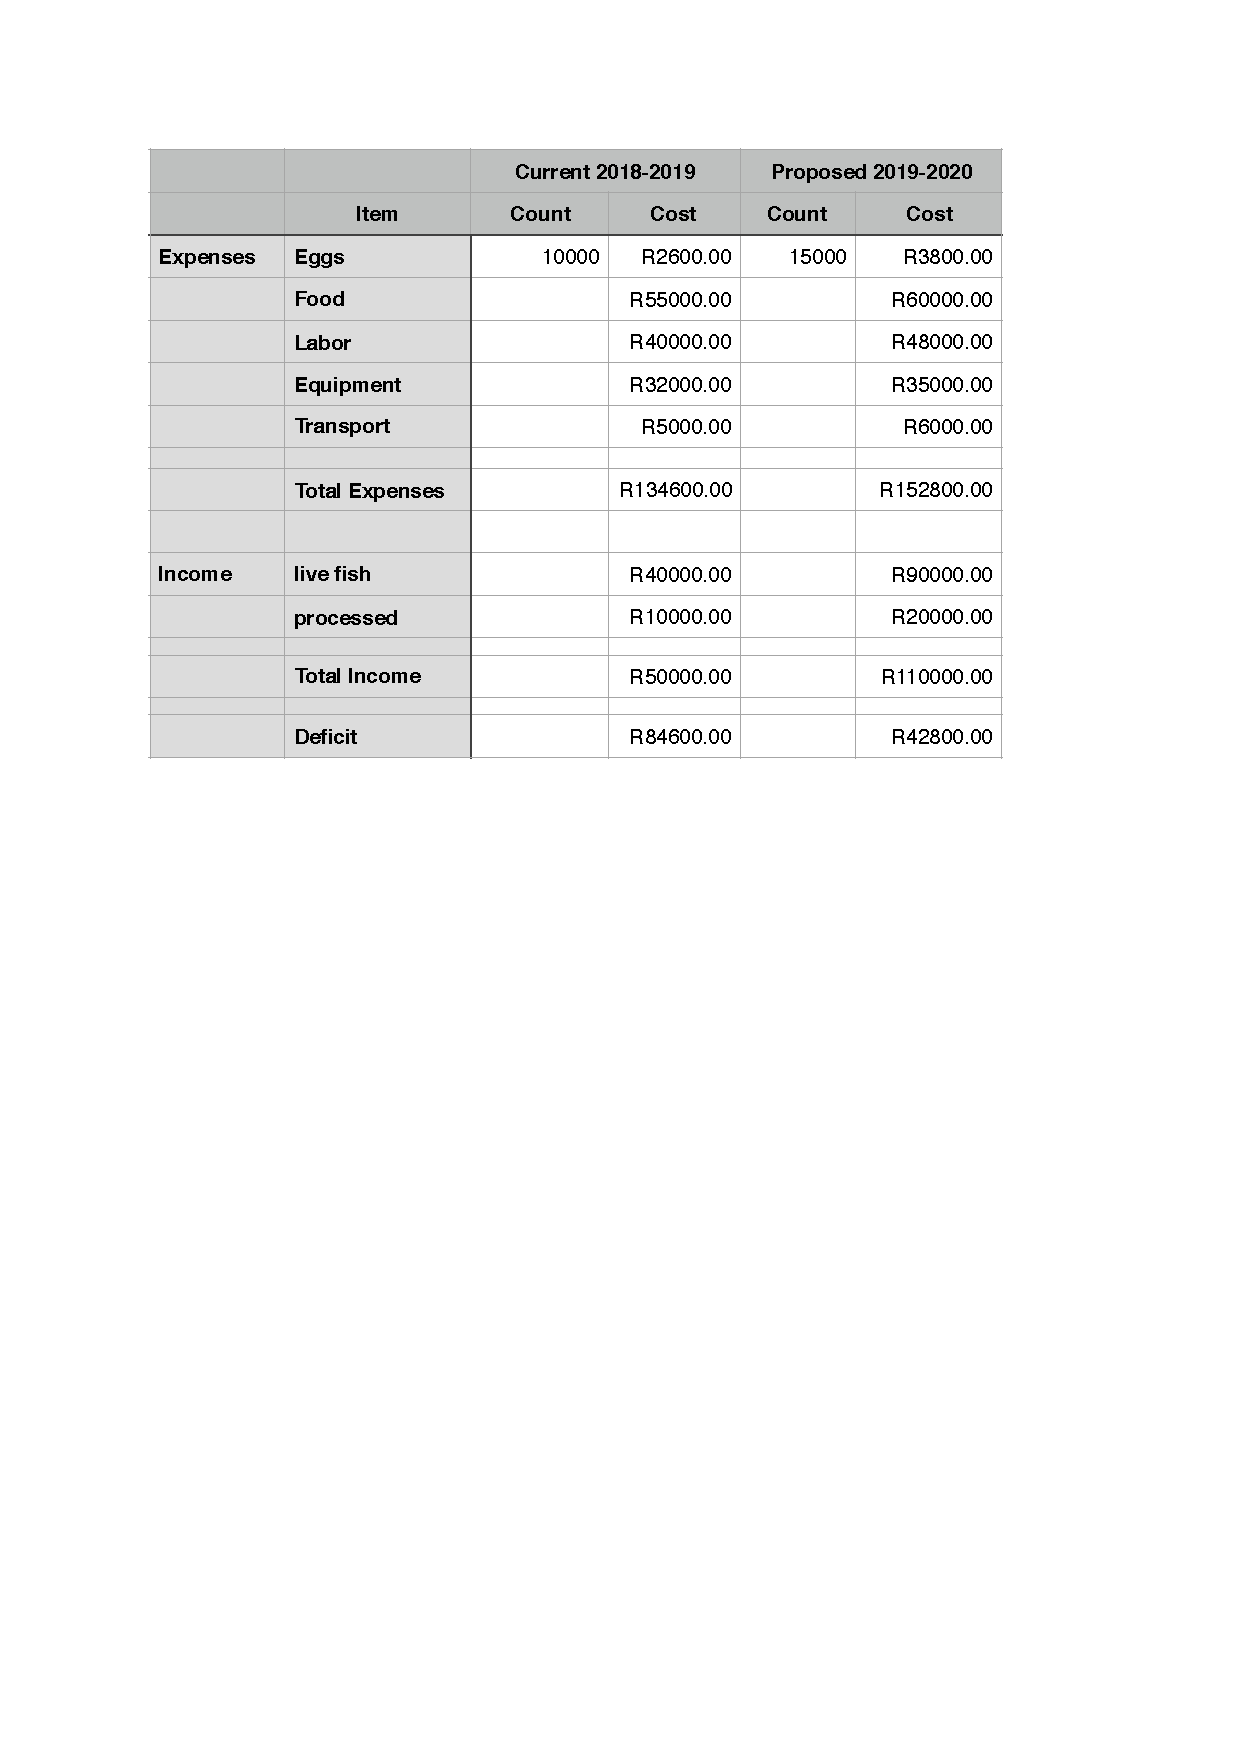
\includegraphics[scale = 0.9]{tables/TablesBudget.pdf}
   \caption{Possible Budget proposal for next season.}
  \label{tab:Budget}
\end{table}
 


